% !TeX spellcheck = cs_CZ
\begin{example}\label{TEO:exam015}
  Metodou smyčkových proudů vyřešme obvod na obr. \ref{es:fig_patocka_topol02}. Řešením se rozumí 
  nalezení velikosti všech šesti proudů \(I_1\), až \(I_6\). Napětí \(U_1\), \(U_2\), \(U_3\) 
  považujme za známá. Příklad bude řešen jen obecně, nejsou zadána konkrétní čísla. Smyslem 
  příkladu je pouze sestavení \(\mathbb{Z}\)-matice obvodu a ukázka kvalitativních vlastností této 
  matice.
  
   {\centering  
    \begin{tabular}{c}
        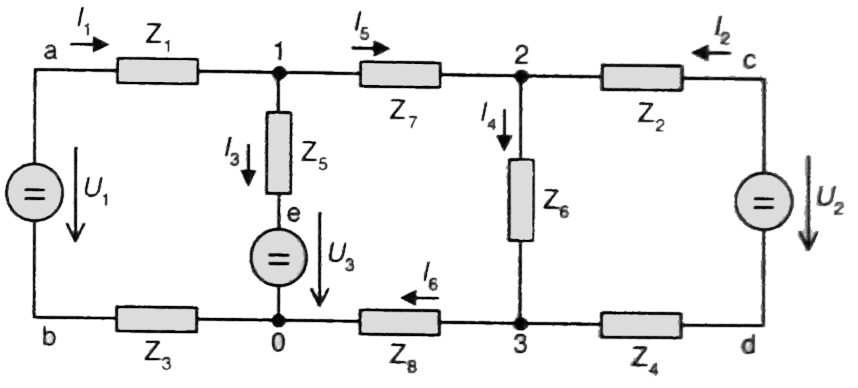
\includegraphics[width=0.7\linewidth]{patocka_topol02a.png}  \\
        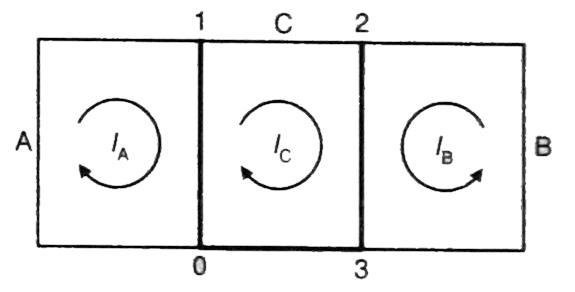
\includegraphics[width=0.7\linewidth]{patocka_topol02b.png}
    \end{tabular}
    \captionsetup{type=figure}
    \captionof{figure}{a) Řešený obvod, b) Úplný strom (silné čáry) a k němu příslušející soustava 
             třech nezávislých smyček \(A\), \(B\), \(C\) se zvolenými směry smyčkových 
             proudů. Každá ze tří nezávislých smyček \(A\), \(B\), \(C\) prochází alespoň 
             jednou nezávislou hranou (slabé čáry), která nepatří do úplného stromu. 
             \cite[s.~43]{Patocka4}} 
    \label{es:fig_patocka_topol02}
  \par}
  
  Obvod má následující parametry:
  \begin{itemize}\addtolength{\itemsep}{-0.2\baselineskip}
   \item Počet uzlů: \(q + 1 = 4\)
   \item Počet hran úplného stromu: \(q = 3\) (tři silně vytažené čáry)
   \item Počet hran (počet neznámých proudů): \(p = 6\)
   \item Počet nezávislých smyček (nezávislých hran): \(n=p-q=3\)
  \end{itemize}
  
  Pro tři nezávislé smyčky \(A\), \(B\), \(C\) lze sestavit soustavu tří rovnic o třech nově 
  zavedených neznámých fiktivních smyčkových proudech \(I_A\), \(I_B\), \(I_C\). Celková napájecí 
  napětí v každé smyčce jsou označena \(U_A\), \(U_B\), \(U_C\):
  \begin{align}\label{ES:eq_topol01}
    U_A &= U_1-U_3 = (Z_1 + Z_3)I_A +Z_5(I_A - I_C)           \nonumber\\
    U_B &= U_1     = (Z_2 + Z_4)I_B+Z6(I_B + I_C)             \nonumber\\
    U_C &= U_3     = (Z_7 + Z_8)I_C+Z_5(I_C - I_A)+Z_6(I_B+I_c)  
  \end{align}
  Přičemž zřejmě platí:
  \begin{subequations}
    \begin{align}\label{ES:eq_topol02}
     I_1 &= I_A,       \qquad\quad\; I_3 = I_A - I_C,                   \\
     I_4 &= I_B + I_C, \quad I_5 = I_C, \quad I_6 = I_C
    \end{align}
    \end{subequations}
  Pravé strany v soustavě rovnic (\ref{ES:eq_topol01}) uspořádáme podle smyčkových proudů do   
  matice ve tvaru tvaru
  \begin{equation}\label{ES:eq_topol03}
   \left(
     \begin{array}{cccc}
       Z_1+Z_3+Z_5  &              &-Z_5  \\
                    & Z_2+Z_4+Z_6  & Z_6  \\
               -Z_5 & Z_6          & Z_5+Z_6+Z_7+Z_8 
     \end{array}
   \right) 
  \end{equation}
  Další postup by byl následující: \emph{Cramerovým pravidlem} rutinně vyřešit tuto soustavu tří 
  rovnic pro tři neznámé smyčkové proudy a dodatečně dopočítat dvě rovnice (\ref{ES:eq_topol02}). 
  Zbývající čtyři identity v soustavě (\ref{ES:eq_topol02}) není nutno počítat. Tím by byl obvod 
  vyřešen. Smyslem příkladu však nebylo vlastní řešení, nýbrž konkrétní ukázka velice zajímavého 
  jevu: matice (\ref{ES:eq_topol03}) je symetrická podle hlavní diagonály. Symetrie matice je 
  důsledkem principu reciprocity, který bude diskutován v následujících kapitolách.
\end{example}